\scanpage{48}

U N I V E R S I T E\par
DES SCIENCES ET TECHNIQUES\par
\uline{DU LANGUEDOC}\par
AMC/MD

Montpellier, le 19 juin 1975

\uline{Diffusion} : Liste A\par
n° 3979

AVIS DE SOUTENANCE D'UNE THESE DE DOCTORAT DE\par
\uline{SPECIALITE BIOLOGIE ANIMALE}

\uline{Nom et prénom du candidat} : MARTEAU Marie

\uline{Titre de la thèse} : Systématique et biologie des acanthocéphales du genre
CORYNOSOMA LUHE 1904.

\uline{Date, heure et lieu de soutenance prévus} : Jeudi 26 juin à 10 heures, salle de
cours n° 5 - U.S.T.L.

\uline{Nom des Directeurs de thèse} : M. EUZET - M. GOLVAN

\uline{Désignation du laboratoire où la thèse est préparée} : Laboratoire de parasitologie
comparée U.S.T.L. et laboratoire de parasitologie C.H.U. St Antoine PARIS.

\uline{Analyse de l'ouvrage} : L'étude anatomique des Acanthocéphales du genre \uline{Corynosoma}
permet de reprendre la systématique des espèces décrites. On démontre que l'on
peut séparer les espèces parantes de cetacés et celles qui vivent dans les
oiseaux marins. On reprend le cycle biologique des Corynosoma et on discute
le phénomène de capture par les poissons. On émet une hypothèse sur la phyllogenèse
des espèces étudiées.

\uline{Durée approximative des recherches ayant abouti à la thèse} : 2 ans

\uline{Composition du jury proposé} :\quad\begin{tabular}[t]{l}M. EUZET\\M. BOUIX\\M. CHABAUD\\M. GOLVAN\end{tabular}

Le Secrétaire Général,

\unsure{E. Siau}
\figure{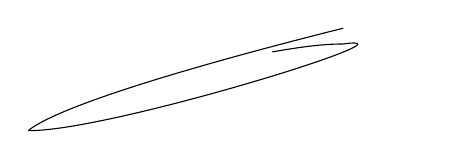
\begin{tikzpicture}[x=1cm,y=1cm]
\draw (0,0) .. controls(.5,.4) and(3,1.05)..(4,1.3);
\draw (0,0).. controls(1,-.02)and(5.1,1.25)..(4.0,1.1)..controls(3.7,1.1)and(3.4,1.05)..(3.1,1.0);
\end{tikzpicture}}
\uline{E. SIAU}

\begin{tabular}{ll}
MR\quad LE PROFESSEUR GROTHENDIECK A.&\\[1em]
MATHEMATIQUES&5-856
\end{tabular}

\mspage{47}
